\documentclass [11pt,twoside]{article}
\usepackage[utf8]{inputenc}
\usepackage[T1]{fontenc}

%Page margins, header and footer positions
\usepackage{geometry}
 \geometry{
 a4paper,
 total={210mm,297mm},
 left=25mm,
 right=25mm,
 top=30mm,
 bottom=25mm,
 headsep=7mm}

\interfootnotelinepenalty=10000

%To display filling dots in the TOC for all entries
\usepackage[titles]{tocloft}
\renewcommand{\cftsecleader}{\cftdotfill{\cftdotsep}}

%Define new header and footer style
\usepackage{fancyhdr}

\pagestyle{fancy}
\fancyhf{}
\lfoot{\textcolor{Gray}{\small{Copyright © 2018, Alessandrelli Caraffa Bionda – All rights reserved}}}
\rfoot{\textcolor{Gray}{\thepage}}
\renewcommand{\headrulewidth}{0pt}

%PACKAGES
\usepackage{wasysym}
\usepackage{pifont}

\newcommand{\supported}{\ding{52}\xspace}
\newcommand{\unsupported}{\ding{55}\xspace}
\newcommand{\partsupported}{\textcolor{black!40}{\ding{52}}\xspace}
\newcommand{\lowsupported}{\textcolor{black!20}{\ding{52}}\xspace}
\newcommand{\unknowsupported}{\textbf{?}\xspace}

%Font: Times
\usepackage{times}
%Change monospaced font
\renewcommand{\ttdefault}{lmtt}

%tables
\usepackage{tabu}
\usepackage{tabularx}
\usepackage{ltablex}
\usepackage{longtable}
\usepackage{float} % To allow the use of H modifier in long tables

%landscape mode
\usepackage{pdflscape}
\usepackage{rotating}
\usepackage{caption}

%make landscape mode be sensitive to even and odd pages
%start
\def\myrotate{\ifodd\c@page\else-\fi 90}
\makeatletter
\global\let\orig@begin@landscape=\landscape%
\global\let\orig@end@landscape=\endlandscape%
\gdef\@true{1}
\gdef\@false{0}
\gdef\landscape{%
    \global\let\within@landscape=\@true%
    \orig@begin@landscape%
}%
\gdef\endlandscape{%
    \orig@end@landscape%
    \global\let\within@landscape=\@false%
}%
\@ifpackageloaded{pdflscape}{%
    \gdef\pdf@landscape@rotate{\PLS@Rotate}%
}{
    \gdef\pdf@landscape@rotate#1{}%
}
\let\latex@outputpage\@outputpage
\def\@outputpage{
    \ifx\within@landscape\@true%
        \if@twoside%
            \ifodd\c@page%
                \gdef\LS@rot{\setbox\@outputbox\vbox{%
                    \pdf@landscape@rotate{-90}%
                    \hbox{\rotatebox{90}{\hbox{\rotatebox{180}{\box\@outputbox}}}}}%
                }%
            \else%
                \gdef\LS@rot{\setbox\@outputbox\vbox{%
                    \pdf@landscape@rotate{+90}%
                    \hbox{\rotatebox{90}{\hbox{\rotatebox{0}{\box\@outputbox}}}}}%
                }%
            \fi%
        \else%
            \gdef\LS@rot{\setbox\@outputbox\vbox{%
                \pdf@landscape@rotate{+90}%
                \hbox{\rotatebox{90}{\hbox{\rotatebox{0}{\box\@outputbox}}}}}%
            }%
        \fi%
    \fi%
    \latex@outputpage%
}
\makeatother
%end

%graphics
\usepackage{graphicx}
\usepackage[dvipsnames, table]{xcolor}
%If you upload images from PC, you need to insert code for the path here (different for Windows and Unix OS)

%References
%\usepackage{xpatch}
%\usepackage[backend=biber, style=numeric, citestyle=numeric, sorting=none]{biblatex}
%\addbibresource{main.bib}

%Other
\usepackage{ifthen}
\usepackage{xspace}
\usepackage{enumitem}
\usepackage{amssymb}
\usepackage[pdftex, colorlinks]{hyperref}
\newcommand{\comment}[1]{{\color{Red}$\blacktriangleright$ Comment: #1 $\blacktriangleleft$}}


% Some utilities\ldots
\usepackage{soul}
\usepackage{tikz}

\usetikzlibrary{calc}
\usetikzlibrary{decorations.pathmorphing}


\makeatletter

\newcommand{\defhighlighter}[3][]{%
  \tikzset{every highlighter/.style={color=#2, fill opacity=#3, #1}}%
}

\defhighlighter{yellow}{.5}

\newcommand{\highlight@DoHighlight}{
  \fill [ decoration = {random steps, amplitude=1pt, segment length=15pt}
        , outer sep = -15pt, inner sep = 0pt, decorate
       , every highlighter, this highlighter ]
        ($(begin highlight)+(0,8pt)$) rectangle ($(end highlight)+(0,-3pt)$) ;
}

\newcommand{\highlight@BeginHighlight}{
  \coordinate (begin highlight) at (0,0) ;
}

\newcommand{\highlight@EndHighlight}{
  \coordinate (end highlight) at (0,0) ;
}

\newdimen\highlight@previous
\newdimen\highlight@current

\DeclareRobustCommand*\highlight[1][]{%
  \tikzset{this highlighter/.style={#1}}%
  \SOUL@setup
  %
  \def\SOUL@preamble{%
    \begin{tikzpicture}[overlay, remember picture]
      \highlight@BeginHighlight
      \highlight@EndHighlight
    \end{tikzpicture}%
  }%
  %
  \def\SOUL@postamble{%
    \begin{tikzpicture}[overlay, remember picture]
      \highlight@EndHighlight
      \highlight@DoHighlight
    \end{tikzpicture}%
  }%
  %
  \def\SOUL@everyhyphen{%
    \discretionary{%
      \SOUL@setkern\SOUL@hyphkern
      \SOUL@sethyphenchar
      \tikz[overlay, remember picture] \highlight@EndHighlight ;%
    }{%
    }{%
      \SOUL@setkern\SOUL@charkern
    }%
  }%
  %
  \def\SOUL@everyexhyphen##1{%
    \SOUL@setkern\SOUL@hyphkern
    \hbox{##1}%
    \discretionary{%
      \tikz[overlay, remember picture] \highlight@EndHighlight ;%
    }{%
    }{%
      \SOUL@setkern\SOUL@charkern
    }%
  }%
  %
  \def\SOUL@everysyllable{%
    \begin{tikzpicture}[overlay, remember picture]
      \path let \p0 = (begin highlight), \p1 = (0,0) in \pgfextra
        \global\highlight@previous=\y0
        \global\highlight@current =\y1
      \endpgfextra (0,0) ;
      \ifdim\highlight@current < \highlight@previous
        \highlight@DoHighlight
        \highlight@BeginHighlight
      \fi
    \end{tikzpicture}%
    \the\SOUL@syllable
    \tikz[overlay, remember picture] \highlight@EndHighlight ;%
  }%
  \SOUL@
}

\makeatother

% Common abbrev. are set as commands to ensure proper spacing after the dot
\RequirePackage{xspace}
\newcommand{\ie}{i.e.\@\xspace}
\newcommand{\aka}{a.k.a.\@\xspace}
\newcommand{\Ie}{I.e.\@\xspace}
\newcommand{\cf}{cf.\@\xspace}
\newcommand{\Cf}{Cf.\@\xspace}
\newcommand{\eg}{e.g.\@\xspace}
\newcommand{\Eg}{E.g.\@\xspace}
\newcommand{\etal}{et al.\@\xspace}
\newcommand{\etc}{etc.\@\xspace}
\newcommand{\wrt}{w.r.t.\@\xspace}
\newcommand{\Wrt}{W.r.t.\@\xspace}



\date{}

\usepackage{placeins}
\usepackage{graphicx,color,listings}
\usepackage{float}
\usepackage[export]{adjustbox}
\usepackage{hyperref}% http://ctan.org/pkg/hyperref
\hypersetup{%
  colorlinks = true,
  linkcolor  = black
}
\usepackage{sectsty}


\sectionfont{\huge}
\subsectionfont{\LARGE}
\subsubsectionfont{\Large}



\begin{document}



%TITLE PAGE

\begin{titlepage}

%LOGO
\centering
{\textcolor{Blue}{\LARGE  {POLITECNICO DI MILANO}}}\\[0.5CM]
\Large {School of Industrial and Information Engineering}\\[0.3CM]
\textbf{\Large Computer Science and Engineering}\\
[1cm]
\begin{figure}[H]
\centering

\includegraphics[scale = 0.3]{Images/Logo/logo.jpg}\\
[1cm]
\end{figure}
{\fontsize{35}{35} \selectfont{\textcolor{Blue}{\textsc{\bfseries  TrackMe RASD}}}}\\[0.5cm]
{\fontsize{25}{70} \selectfont{\textcolor{Blue}{\textbf{{Requirements Analysis and Specification
        Document}}}}}\\[0.5cm]     
{\textcolor{Black}{\LARGE{Software Engineering 2 Project}}}\\ [2cm]     
\centering
The project was made by\\[0.5cm]
\textbf {\LARGE Luca Alessandrelli 846260}\\[0.2cm]
\textbf {\LARGE Andrea Caraffa 919970}\\[0.2cm]
\textbf {\LARGE Andrea Bionda 921082}\\[0.5cm]
Version 1.0  -  2018/2019
\end{titlepage}

%Define deliverable specific info
%Replace cell contents where needed
\begin{table}[h!]
\begin{tabu} to \textwidth { X[0.3,r,p] X[0.7,l,p] }
\hline

\textbf{Deliverable:} & RASD\\
\textbf{Title:} & Requirements Analysis and Specification Document \\
\textbf{Authors:} & Luca Alessandrelli, Andrea Caraffa, Andrea Bionda \\
\textbf{Version:} & 1.0 \\ 
\textbf{Date:} & 19-October-2018 \\
\textbf{Download page:} & https://github.com/lucaalessandrelli/AlessandrelliCaraffaBionda.git \\
\textbf{Copyright:} & Copyright © 2017, Luca Alessandrelli, Andrea Caraffa, Andrea Bionda – All rights reserved \\
\hline
\end{tabu}
\end{table}




\setcounter{page}{2}


%------------------------------------------------------------------------------------------------------------------------------------------------
\newpage
\addcontentsline{toc}{section}{Table of Contents}
\tableofcontents
\newpage
\addcontentsline{toc}{section}{List of Figures}
\listoffigures
\addcontentsline{toc}{section}{List of Tables}
\listoftables

%------------------------------------------------------------------------------------------------------------------------------------------------
\clearpage
{\color{Blue}{\section{Introduction}}}
\label{sect:introduction}
\subsection{Purpose}
... Here you see a subsubsection
\subsection{Scope}
... Here you see a subsubsection
\subsubsection{Goals}

\begin{enumerate}
\item[•] {\Large Data4Help}
	\begin{enumerate}
		\item [G.1] Locate users' position on demand and in real time.
		\item [G.2] Retrieve users’ health status on demand and track it in live.
		\item [G.3] Allow third parties registered to retrieve information about users in 				single mode and in group mode.
		\item [G.4] Ensure users' privacy.
		\item [G.5] Allow third parties to retrieve historical data and statistics about 				users.
	\end{enumerate}
	
\item[•] {\Large AutomatedSOS}
	\begin{enumerate}
		\item [G.1] Monitor in real time users’ health status with more attention to 					critical parameters.
		\item [G.2] Allow only health-interested third parties the access to data detected 				by AutomatedSOS.
		\item [G.3] Provides to send an ambulance if certain parameters are below critical 				values.
	\end{enumerate}
	
\item[•] {\Large Track4Run}	
	\begin{enumerate}
		\item [G.1] Allow races organizer to promote into the system a new race and specify 			all the useful information about the race.
		\item [G.2] Allow users to enrol on a specific race.
		\item [G.3] Allow users to watch in real time the position of every athletes in a 				specific race during the run.
	\end{enumerate}
\end{enumerate}

\subsubsection{World Phenomena}
... what are world phenomenass???

\subsection{Definitions, Acronyms, Abbrevations}

\begin{enumerate}
\item[•] {\Large Definitions}
	\begin{enumerate}
		\item User: authenticated individual that provides information about himself
		\item Third party society: external society interested to retrieve data from 					TrackMe's user.
		\item Single mode: data acquisition from a specific registered individual.
		\item Group mode: data acquisition from many individuals. 
		\item Live acquisition: third parties can access to data as soon they are ready, 				through service updates.
		\item On demand acquisition: third parties can access to data when they request 				them.
		\item Subscribers: third parties allowed to receive live acquisition about 						preselected	group.
		\item User credentials: information that an individual has to provide to become a 				registered user: name, surname, date of birth, address, email, telephone
			number, job, marital status and fiscal code. 
		\item Third parties’ credentials: information that a company has to provide to 					become a registered one: company name, p.iva.
		\item Race information: all the information about the run: name, date, promoters, 				maximum number of participants and race path.
	\end{enumerate}
\end{enumerate}
	
\subsection{Revision History}
... Here you see a subsubsection
\subsection{Reference Documents}
... Here you see a subsubsection
\subsection{DocumentStructure}
... Here you see a subsubsection

%what you write here is a comment that is not shown in the final text

%------------------------------------------------------------------------------------------------------------------------------------------------
\clearpage
{\color{Blue}{\section{Overall Description}}}
\label{sect:overview}
\subsection{Product perspective}
The following Class Diagrams represent the three services and the domain model where they work.
White class are dedicated to perform Data4Help service, the other two applications are listed below.
\begin{figure}[H]
\centering
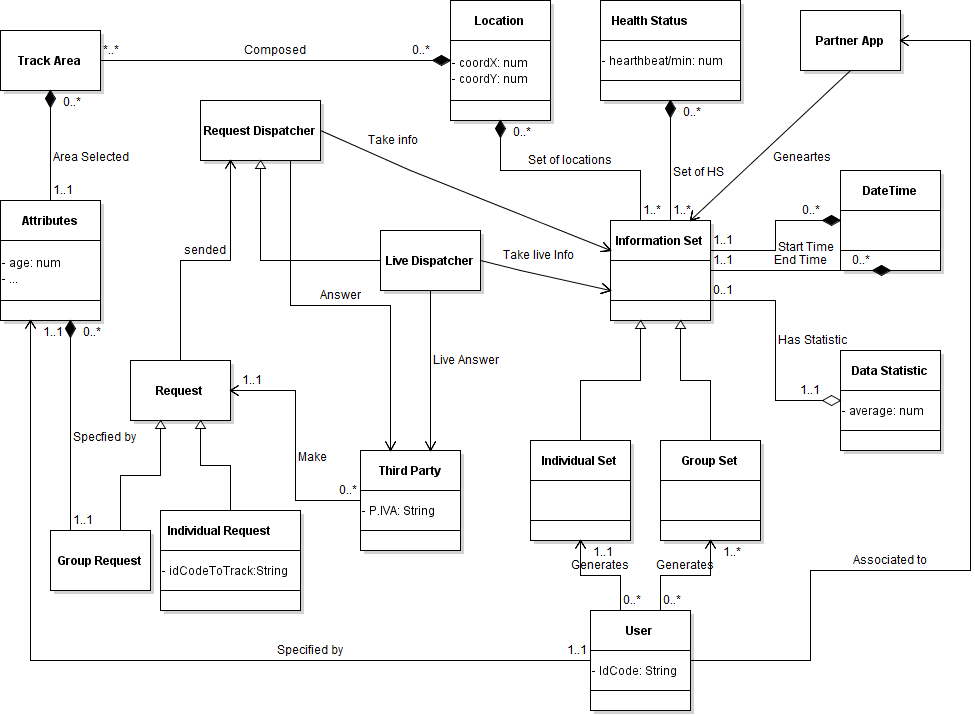
\includegraphics[scale=0.45]{Images/Class_Data4Help.png}
\caption{Data4Help Class Diagram}
\end{figure}
\noindent
{\color{Salmon} Red classes} are dedicated to {\color{Salmon} AutomatedSOS} application, supported by Data4Help service (white ones).
\begin{figure}[H]
\centering
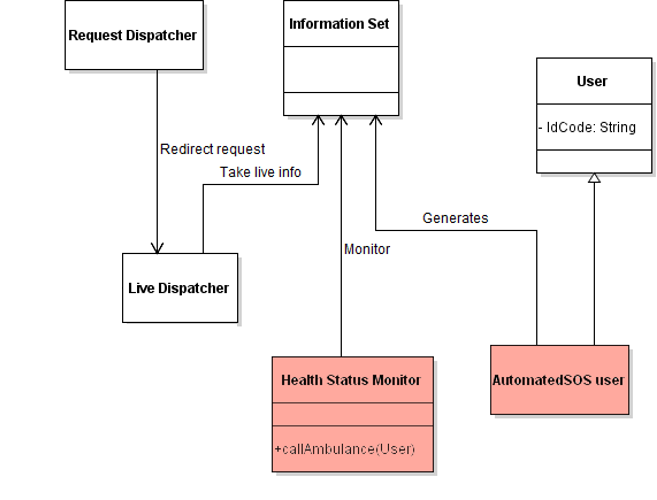
\includegraphics[scale=0.48]{Images/Class_AutoSOS.png}
\caption{AutomatedSOS Class Diagram}
\end{figure}

\begin{minipage}{\textwidth}
{\color{LimeGreen} Green classes} are dedicated to {\color{LimeGreen} Track4Run} application, supported by Data4Help service (white ones).
\begin{figure}[H]
\centering
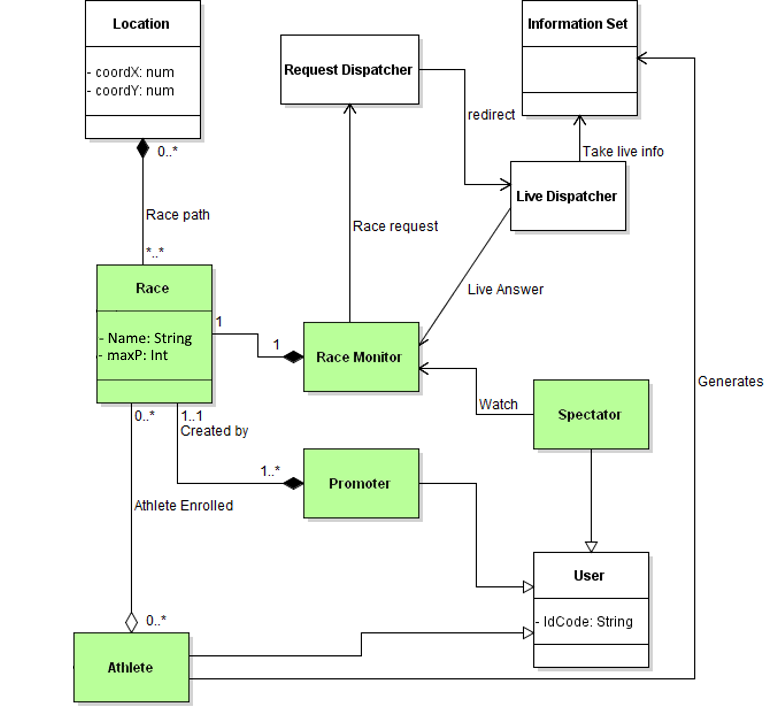
\includegraphics[scale=0.7]{Images/Class_Track4Run.png}
\caption{Track4Run Class Diagram}
\end{figure}
The following State Chart represents the behaviour of a Data Request Object.
\begin{figure}[H]
\centering
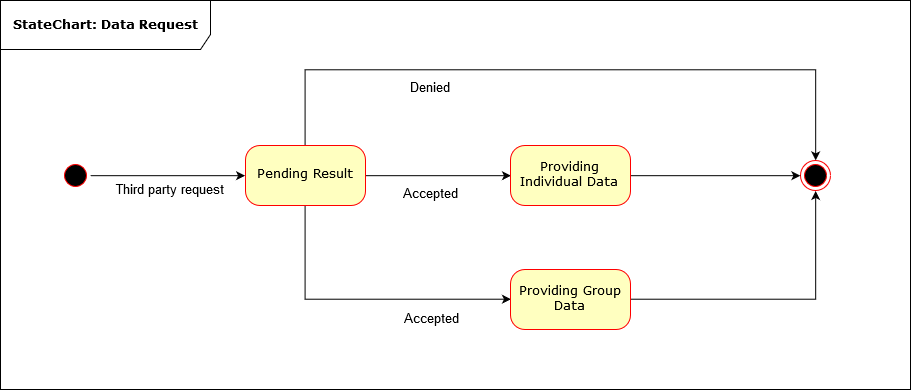
\includegraphics[scale=0.5]{Images/StateChart.png}
\caption{Data Request Object State Chart}
\end{figure}
\end{minipage}

\subsection{Product functions}
The system-to-be under analysis have to offer several functions. Below, the main functions provided by each services are more precisely specified, considering all the aspects emerged from the previous list of goals.
\subsubsection{Data4Help - Providing data to third parties }
This is the core function that Data4Help has to ensure. After collecting users position and health status information from external partner applications, Data4Help provides these data to the third party interested in having them. Data4Help provides data on demand sending to the third party all the available data about an individual (or a group of individual) collected so far. The third party is provided with all the data about a user collected until time of the data request. In addition, Data4Help offers a providing data service in real time, allowing the third party to subscribe to new data and to receive them as soon as they are produced. TrackMe in order to offer a complete solution to third parties send them also statistics about data.

\subsubsection{AutomatedSOS - Sending ambulance request in critical situation}
AutomatedSOS monitors the health status of the subscribed customers and, when such parameters are below certain threshold, sends to the location of the customer an ambulance, guarantying a reaction time of less than 5 seconds from the time parameters are below the threshold.
\bigbreak
\noindent
Therefore, the main function offered by AutomatedSOS is sending an ambulance request, with the relative user position, to the nearest hospital to the user. In order to optimize the times, the ambulance request contains all the data about the user health status. Providing these information, when rescue arrives, it can immediately act accordingly to the received data. AutomatedSOS retrives data directly from the user's smartwatch and send them to Data4Help. In order to keep under control the user's health status AutomatedSOS performs monitoring using these retrieved data and other hystorical data got from Data4Help, the latter are used to have a profile of the user's health status.
\subsubsection{Track4Run - Run management}
Track4Run offers three different functionality for its users, which can be all grouped under the 'run management' function. A user can be a promoter, in this case the user can create the event run , which will be visible to every other users. Once created a run, the promoter can define the path in an interactive way, that is by drawing the path directly on a map. Track4Run allows the promoter to set other additional information, like the start time or an overall description of the run. Finally, the promoter can invite to the run all the participants. Every run can be enrolled by everyone, so the scope of inviting a person is just to promote the run and to facilitate the enrollment process.
\bigbreak
\noindent
The athletes have to be user too. Once received a run request, the athlete can enroll to the run or reject it. In the first case, Track4Run tracks in real time the participant position for all the run through a smartwatch. 
\bigbreak
\noindent
A user can also be a simple spectator and see on a map the position of all runners during the run. A spectator is provided with the main information about the participants and with live time laps.

\subsection{User characteristics}
\begin{enumerate}
\item Third Party: Company interested in retrieving useful data from TrackMe's users. Usually, this information can be relevant for marketing strategy.

\item User: Individual whose data are acquired from TrackMe through Data4Help service and are provided to third parties. AutomatedSOS is a service thought for elderly people, while Track4Run is a service thought for athletes, promoters and spectators of runs. User's privacy is protected by each service.

\end{enumerate}

\subsection{Assumptions, dependencies and constraints}
In the specification document certain parts are not specified and a bit ambiguous. Therefore, we decided to make the following assumptions.

\subsubsection{Text Assumptions}
\begin{enumerate}

\item[•] {\Large Data4Help}
	\begin{enumerate}
	\item User's data are collected from partner applications or from the other two TrackMe applications installed on user's devices.
	\item Partner applications can be all the sport assistant apps, GPS assistant apps or all the other applications that can retrieve location and health status of individual for such reason.
	\item All the partner applications require to submit user credentials. 
	\item When the partner application is installed and credentials are submitted,
	the user is required to accept privacy policy, composed in two parts:
		\begin{enumerate}
		\item The first, mandatory, user accept to be tracked in group mode.
		\item The second, optional, user accept to be tracked in single mode.
		\end{enumerate}
	\item Individual monitoring requests are not accepted or denied one by one by the specific user. If the user agreed on the treatment of his data as information of an individual (second part of privacy policy) all individual monitoring request by third parties are automatically accepted.	
	\item Data are collected from partner application only when they are active on user's device.
	\item Only third parties that are registered to Data4Help can request the monitoring service.
	\item Groups are characterized by its members' attributes (age, gender, city, …).
	\item Health status parameters that can be acquired are all the ones supported by a standard smartwatch as: Heart Rate, Blood Pressure, Pedometer, Calories Calculation.
	\item The answers to both Individual Monitoring Requests and Group Monitoring Requests contain also some statistics other than raw data.
	\item Live acquisition request expires after one month from the moment that is formulated.
	\end{enumerate}
	
\item[•] {\Large AutomatedSOS}
	\begin{enumerate}
	\item AutomatedSOS exploit only smartwatches devices to retrieve all the information needed.
	\item AutomatedSOS is an application that needs to be installed into the user's device.
	\item All data retrieved by AutomatedSOS are sent to Data4Help.
	\item In any case, data retrieved by AutomatedSOS will not be sent to third parties if they perform an individual request. Thus TrackMe does not offer additional services for third parties through AutomatedSOS.
	\item In order to keep under systematic review the user's health status and have a broad view of it, some historical information about the user are periodically received by Data4Help's Database.
    \item This service can be used only by elderly people (70+) or by who really need it, in order to avoid useless waste of resources.
    \item User can see all personal information that have been sent to the Data4Help service. 
	\end{enumerate}
	
\item[•] {\Large Track4Run}
	\begin{enumerate}
	\item During the registration to the application the user is asked to accept or deny the treatment of his data by  Data4Help service.
	\item The application has three functions: 
	\begin{enumerate}
	\item Promoter: allow the user to manage a run.  
	\item Athlete: allow the user to participate to a run. In order to be an athlete the request of data treatment by the Data4Help service need to be accepted.
	\item Spectator: Allow the user to watch in real time the positions of all the athletes in a given run.
	\end{enumerate}
	\item All run events are seen as public runs, so every user can enroll to future runs.
	\item Any user can organize an event and also invite other users to enroll to the run.
    \item All the events can be spectated by users.
    \item All users invited to a run can accept or discard the request.
    \item Run paths are always composed by citizen routes (never in private circuits or stadiums)
    \end{enumerate}
\end{enumerate}

\subsubsection{Domain Assumptions}
\begin{enumerate}

\item[•] {\Large Data4Help}
	\begin{enumerate}
	\item [D.1] User's information are collected from partner applications or from the other two TrackMe applications installed on users' devices.
	\item [D.2] All the partner applications require to submit user credentials.
	\item [D.3] The identification (fiscal code, social security number) and the secondary data (attributes) given by the individual during the registration are correct.
    \item [D.4] Devices used to monitor individuals always report correct values.
    \item [D.5] Partner application always report correct values to Data4Help.
	\item [D.6] In order to perform an individual request, third parties has to know the user's fiscal code or security number.
	\item [D.7] Security number and fiscal code are not information given to third parties by Data4Help.
	\end{enumerate}
	
\item[•] {\Large AutomatedSOS}
	\begin{enumerate}
	\item [D.4] Devices used to monitor individuals always report correct values.
	\item [D.9] The user always dresses a smartwatch on which AutomatedSOS is installed and running.    
	\item [D.10] The first aid system is always up and ready to receive messages from AutomatedSOS.
    \item [D.11] The ambulance successfully reach the location of the individual.
    \item [D.12] The ambulance always get to the location in the minimum amount of time.
    
	\end{enumerate}
	
\item[•] {\Large Track4Run}
	\begin{enumerate}
	\item [D.4] Devices used to monitor individuals always report correct values.
	\item [D.13] During a run athletes always wear a smartwatch on which Track4Run is installed.
	\item [D.14] The path defined by the organizer actually exist.
    \item [D.16] If an athlete enroll to a run then athlete also participates to the run.
    \item [D.17] All athletes have their tracking devices with them and the application is enabled for the entire duration of the run.
    \item [D.18] Athletes never go out of the defined path.
	\end{enumerate}
\end{enumerate}

%------------------------------------------------------------------------------------------------------------------------------------------------
\clearpage
{\color{Blue}{\section{Specific Requirements}}}
\label{sect:requirements}
Organize this section according to the rules defined in the project description. 
\subsection{External Interface Requirements}
\subsubsection{User Interfaces}
\subsubsection{Hardware Interfaces}
\subsubsection{Software Interfaces}
\subsubsection{Communication Interfaces}


\subsection{Functional Requirements}
\begin{enumerate}
\item[•]{\Large Data4Help}
	\begin{enumerate}
	\item [G.1] \textbf{Collect users' position and health status.}
		\begin{enumerate}
		\item [D.1] Users' information are collected from partner applications or from the other two TrackMe applications installed on users' devices.
		\item [D.2] All the partner applications require to submit user credentials.
		\item [D.3] The identification (fiscal code, social security number) and the secondary data (attributes) given by the individual during the registration are correct.
		\item [R.1] Retrieve user credentials inserted into partner application as group attributes.
		\item [R.2] Allow users already registered in Data4Help world to sign in with his account without provide user credentials again.
		\item [R.3] Allow individuals to agree with privacy policy (first part). Registered users, now, can be tracked in group mode request through installed application.  
		\item [R.4] Allow individuals to specify, during registration, if they are also interested to be tracked in single mode request (second part) through installed application.  .
		\item [D.4] Devices used to monitor individuals always work and report 			the correct values.	
    	\item [D.5] Partner application always report correct values to Data4Help.
    	\item [R.5] The system has to correctly receive data from partner applications installed on users' device.
    	\end{enumerate}	
    	
    \item [G.2] \textbf{Provide to Third Parties, the users' position and heath status.}
    	\begin{enumerate} 
    	\item [R.6] Allow third parties registration to Data4Help service, where they have to specify all their credentials.
    	\end{enumerate}	
		
		\begin{enumerate} 
		\item [G.2.1] \textbf{Provide data on-demand to non-subscribed third parties.}
		\begin{enumerate} 
		\item [R.7] For each user registered ,the system has to automatically retrieve and store data from partner applications with a resolution of 10 minutes.	
		\item [R.8] The system has to collect inside his database all the useful information that match the request.
		\item [R.9] The system has to send to applicant all the data already collected.
    	\end{enumerate}	
    	
    	\item [G.2.2] \textbf{Provide data in real-time to subscribed third parties.}
		\begin{enumerate}
		\item [D.8] Live acquisition lasts 24 hours to reduce waste of resources.
    	\item [R.10] Allow third parties subscription to interested group in order to receive live data.
    	\item [R.11] When a real time request is performed the system has to collect and store specific users' data with a resolution of 1 minute.
    	\item [R.12] Provide to subscribed third parties data as soon as they are available by the system.
    	\end{enumerate}
    	\end{enumerate}
    
	\item [G.3] \textbf{Allow third parties two different ways to get users' data.}
		\begin{enumerate}     
    	\item [G.3.1] \textbf{Allow third parties to get data of a single person.}
		\begin{enumerate}
		\item [D.6] In order to perform an individual request, third parties has to know the user's fiscal code or security number.
		\item [D.7] Security number and fiscal code are not information given to third parties by Data4Help.
    	\item [R.13] Allow third parties to insert fiscal code of user that want to track.
    	\item [R.14] Deny third parties to receive information about users in  single mode, that have not accepted second part of privacy policy.
    	\item [R.15] Collect all the useful information retrieved by Data4Help that are produced by the interested users 
    	\item [R.16] Send all the collected information to request applicant.
    	\end{enumerate}
    
    	\item [G.3.2] \textbf{Allow third parties to get data of a group of people.}
		\begin{enumerate}
    	\item [R.17] Allow third parties to insert attributes in which they are interested to restrict their field of search.
    	\item [R.18] Deny third parties to receive information if the provided information can hurt users' privacy, for this purpose group request under 1000 users involved are rejected.
    	\item [R.15] Collect all the useful information retrieved by Data4Help that are produced by the interested users 
    	\item [R.16] Send all the collected information to request applicant.
    	\end{enumerate}
    	\end{enumerate}
    	
    \item [G.4] \textbf{Provide data in an anonymous way, to protect users' privacy.}
		\begin{enumerate}
    	\item [R.14] Deny third parties to receive information about users in  single mode, that have not accepted second part of privacy policy.
    	\item [R.18] Deny third parties to receive information if the provided information can hurt users' privacy, for this purpose group request under 1000 users involved are rejected.
    	\end{enumerate}	
			
	\end{enumerate}
	
	
\item[•]{\Large AutomatedSOS}
	
	\begin{enumerate}
	\item [G.5] \textbf{Retrieve user's position and health status.}
		\begin{enumerate}
		\item [R.19] Allow users to be tracked from AutomatedSOS filling up the registration and agreeing to both parts of privacy policy.
		\item [D.4] Devices used to monitor individuals always report correct values.
		\item [D.9] The user always dresses a smartwatch on which AutomatedSOS is installed.    
		\item [R.20] The application has to interact with Smartwatch/Smartphone APIs in order to retrieve location and health status.
		\item [R.21] The application is able to send to Data4Help service all the informations already retrieved in live acquisition.
		\end{enumerate}
		
	\item [G.6] \textbf{Allow health-interested third parties the access to data detected by AutomatedSOS.}
		\begin{enumerate}
		\item [R.22] Allow non-profit organizations to register into AutoatedSOS portal and becoming health third parties.
		\item [R.23] Allow health third parties to receive informations about all the users registered to AutomatedSOS through Live Acquisition performed by Data4Help.
		\end{enumerate}
	
	\item [G.7] \textbf{Monitor user's health parameters.}
		\begin{enumerate}
		\item [R.20] The application has to interact with Smartwatch/Smartphone APIs in order to retrieve location and health status.
		\end{enumerate}
		
	\item [G.8] \textbf{Send an ambulance to users' location whenever certain parameters are below the threshold.}
		\begin{enumerate}
		\item [R.24] The application has to control health status with data retrieved in local to realize immediately if certain parameters are critical.
		\item [R.25] The application has to call an ambulance, if parameters are critical.
		\item [D.10] The ambulance system is always up and ready to receive messages from AutomatedSOS.
		\item [R.26] Supply to hospital user's location and all the useful information to provide efficient first aid.
		\item [D.11] The ambulance successfully reach the location of the individual.
		\end{enumerate}
		
  	\end{enumerate}
  	
  	
\item[•]{\Large Track4Run}
	
	\begin{enumerate}
	\item [G.5] \textbf{Retrieve user's position and health status.}
		\begin{enumerate}
		\item [R.27] Allow users to be tracked from Track4Run filling up the registration and agreeing to both parts of privacy policy.
		\item [D.4] Devices used to monitor individuals always report correct values.
		\item [R.20] The application has to interact with Smartwatch/Smartphone APIs in order to retrieve location and health status.
		\item [R.21] The application is able to send to Data4Help service all the informations already retrieved in live acquisition.
		\end{enumerate}
		
	\item [G.9] \textbf{Allow promoters to manage a run.}
		\begin{enumerate}
		\item [R.22] Allow users to create a run providing all the general information about the competition.
		\item [R.23] Allow users to specify if the race is public or private.
		\item [D.4] Devices used to monitor individuals always report correct values.
		\item [D.13] During a run athletes always dress a smartwatch on which Track4Run is installed.
			
		\item [G.9.1] \textbf{Allow promoters to define a path for the run.}
			\begin{enumerate}
			\item [R.24] Allow promoters to define a path for the race by selecting the routes inside a map.
			\item [D.14] The path defined by the organizer actually exist.
			\end{enumerate}
			
		\item [G.9.2] \textbf{Allow promoters to invite athletes to the run.}
			\begin{enumerate}
			\item [R.25] Allow promoters to invite athlete to be runner of their private race.
			\item [R.26] Allow promoters to specify maximum number of athletes that can take part to their public race.
			\end{enumerate}
	\end{enumerate}
	
	\item [G.10] \textbf{Allow athletes to enroll on a specific run.}
		\begin{enumerate}
		\item [R.27] Allow users to see all the public races and private races in which he is invited.
		\item [R.28] Allow user to select a race and add him to the athletes involved.
		\item [D.16] If an athlete enroll to a run then he also participates to the run.
		\end{enumerate}
	
	\item [G.11] \textbf{Allow spectators to watch in real time the position of every athletes in a specific run.}
		\begin{enumerate}
		\item [D.17] All athletes have their tracking devices with them and the application enabled for the entire duration of the run.	
		\item [R.29] Allow user to select a race to be viewed.
		\item [R.30] The application must be able to request to Data4Help the positions of all the other athletes involved.
		\item [R.31] The application must be able to receive and display the positions of all the other athletes involved.
		\item [D.18] Athletes never go out of the defined path.
		\end{enumerate}
	\end{enumerate}

\end{enumerate}

\subsubsection{Use Case Diagram}


\subsubsection{AutomatedSOS Use Cases}
\begin{table}[h]
\begin{tabular}{|l|l|}
\hline
Name             & Sign up \\ \hline
Actors           & User  \\ \hline
Entry Conditions & The User has AutomatedSOS application installed on his/her smartwatch.    \\ \hline
Event Flow       & \parbox{.45\textwidth}{\begin{enumerate}
            \item The user clicks on the "Sing Up" button.
            \item The user accepts the treatment of data policy.
            \item The user fills all the attribute fields and clicks on "Register Now" button.
            \item The system creates the user's account saving his/her attributes.
        \end{enumerate}}\\ \hline
Exit Condition   & The user's account has been created and the user is now registered.\\ \hline
Exceptions       & \parbox{.45\textwidth}  
{\begin{itemize}
\item If the user does not accept the treatment of data policy a warning is generated saying that in order to register the policy must be accepted.
\item If the system notices that the social security number or fiscal code used in a registration are already linked to an existing account then a warning is generated saying that there is already an account registered with the given credentials.
\end{itemize}}\\ \hline
\end{tabular}
\end{table}

\begin{table}[h]
\begin{tabular}{|l|l|}
\hline
Name             & Sign in \\ \hline
Actors           & User  \\ \hline
Entry Conditions & The User has AutomatedSOS application installed on his/her smartwatch.    \\ \hline
Event Flow       & \parbox{.45\textwidth}{\begin{enumerate}
            \item The user clicks on the "Sing In" button.
            \item The user inserts his/her social security number or fiscal code and his/her password, then clicks the "Enter" button.
            \item The system accept the login in request.
        \end{enumerate}}\\ \hline
Exit Condition   & The user's account has been loaded by the app and the user is now logged in.\\ \hline
Exceptions       & \parbox{.45\textwidth}  
{\begin{itemize}
\item If user inserts invalid log in credentials a warning is generated, saying the credentials are invalid.
\end{itemize}}\\ \hline
\end{tabular}
\end{table}

\begin{table}[h]
\begin{tabular}{|l|l|}
\hline
Name             & Monitor data \\ \hline
Actors           & User  \\ \hline
Entry Conditions & The User is logged in. \\ \hline
Event Flow       & \parbox{.45\textwidth}{\begin{enumerate}
            \item The user clicks on the "Monitor Data" button.
            \item The system gets all the information that have been retrieved by the application to the user.
\end{enumerate}}\\ \hline
Exit Condition   & All the information retrieved by the application are shown on the app.\\ \hline
Exceptions       & \parbox{.45\textwidth}  
{\begin{itemize}
\item If the system do not find information about the user then a warning message is shown to the user saying that until now no user data has been recorded by the application.
\end{itemize}}  \\ \hline
\end{tabular}
\end{table}

\begin{table}[h]
\begin{tabular}{|l|l|}
\hline
Name             & Monitor current health status \\ \hline
Actors           & User  \\ \hline
Entry Conditions & The User is logged in. \\ \hline
Event Flow       & \parbox{.45\textwidth}{\begin{enumerate}
            \item The user clicks the "Monitor health status" button.
            \item The system shows all the health values that are being retrieved in real time.
        \end{enumerate}}\\ \hline
Exit Condition   & All the health parameters retrieved by the application are shown on the app in real time.\\ \hline
Exceptions       & \parbox{.45\textwidth}  
{\begin{itemize}
\item If no health parameters are retrieved a warning message is displayed saying to the user he must wear the smartwatch in order to see parameters in real time. \end{itemize}}\\ \hline
\end{tabular}
\end{table}

\subsubsection{Track4Run Use Cases}
\begin{table}[h]
\begin{tabular}{|l|l|}
\hline
Name             & Sign up \\ \hline
Actors           & User  \\ \hline
Entry Conditions & The User has AutomatedSOS application installed on his/her smartwatch.    \\ \hline
Event Flow       & \parbox{.45\textwidth}{\begin{enumerate}
            \item The user clicks on the "Sing Up" button.
            \item The user accepts the treatment of data policy.
            \item The user fills all the attribute fields and clicks on "Register Now" button.
            \item The system creates the user's account saving his/her attributes.
        \end{enumerate}}\\ \hline
Exit Condition   & The user's account has been created and the user is now registered.\\ \hline
Exceptions       & \parbox{.45\textwidth}  
{\begin{itemize}
\item If the user does not accept the treatment of data policy a warning is generated saying that in order to register the policy must be accepted.
\item If the system notices that the social security number or fiscal code used in a registration are already linked to an existing account then a warning is generated saying that there is already an account registered with the given credentials.
\end{itemize}}\\ \hline
\end{tabular}
\end{table}

\begin{table}[h]
\begin{tabular}{|l|l|}
\hline
Name             & Sign in \\ \hline
Actors           & User  \\ \hline
Entry Conditions & The User has Track4Run application installed on his/her smartwatch or smartphone.    \\ \hline
Event Flow       & \parbox{.45\textwidth}{\begin{enumerate}
            \item The user clicks on the "Sing In" button.
            \item The user inserts his/her social security number or fiscal code and his/her password, then clicks the "Enter" button.
            \item The system accept the login in request.
        \end{enumerate}}\\ \hline
Exit Condition   & The user's account has been loaded by the app and the user is now logged in.\\ \hline
Exceptions       & \parbox{.45\textwidth}  
{\begin{itemize}
\item If user inserts invalid log in credentials a warning is generated, saying the credentials are invalid.
\end{itemize}}\\ \hline
\end{tabular}
\end{table}

\begin{table}[h]
\begin{tabular}{|l|l|}
\hline
Name             & Sign in \\ \hline
Actors           & User  \\ \hline
Entry Conditions & The User has Track4Help application installed on his/her smartwatch or smartphone.    \\ \hline
Event Flow       & \parbox{.45\textwidth}{\begin{enumerate}
            \item The user clicks on the "Sing In" button.
            \item The user inserts his/her social security number or fiscal code and his/her password, then clicks the "Enter" button.
            \item The system accept the login in request.
        \end{enumerate}}\\ \hline
Exit Condition   & The user's account has been loaded by the app and the user is now logged in.\\ \hline
Exceptions       & \parbox{.45\textwidth}  
{\begin{itemize}
\item If user inserts invalid log in credentials a warning is generated, saying the credentials are invalid.
\end{itemize}}\\ \hline
\end{tabular}
\end{table}

\begin{table}[h]
\begin{tabular}{|l|l|}
\hline
Name             & Create a run \\ \hline
Actors           & User  \\ \hline
Entry Conditions & The User is logged in.    \\ \hline
Event Flow       & \parbox{.45\textwidth}{\begin{enumerate}
            \item The user clicks on the "Promote a Run" button.
            \item The system show a new tab where the user can define the path, name, date and athletes (other users).
            \item The system create the event and automatically send notifications to all athletes specified by the promoter asking them if they want to participate to the run.
        \end{enumerate}}\\ \hline
Exit Condition   & The run event has been created and is visible in the list of promoted events.\\ \hline
Exceptions       & \parbox{.45\textwidth}  
{\begin{itemize}
\item During the creation of the run the user can cancel the operation and go back to the main menu at any point clicking the "Cancel" button.
\item If the user do not insert critical information like the path, the name and the date a warning message is shown saying that critical parameters are missing in order to create the run. The user can close the warning message and fill the remaining parameters or cancel the operation, going back to the main menu.
\item The system needs to do something if the defined path cannot be a real path for the run??
\end{itemize}}\\ \hline
\end{tabular}
\end{table}


\subsection{Performance Requirements}

\subsection{Design Constraints}
\subsubsection{Standards compliance}
\subsubsection{Hardware limitations}
\subsubsection{Any other constraint}

\subsection{Software System Attributes}
\subsubsection{Reliability}
\subsubsection{Availability}
\subsubsection{Security}
\subsubsection{Maintainability}
\subsubsection{Portability}


%------------------------------------------------------------------------------------------------------------------------------------------------
\clearpage
{\color{Blue}{\section{Formal Analysis Using Alloy}}}
\label{sect:alloy}
\subsection{Code}
\lstinputlisting[language=alloy]{Files/alloyCode.als}

\subsection{Results}
\begin{figure}[H]
\centering
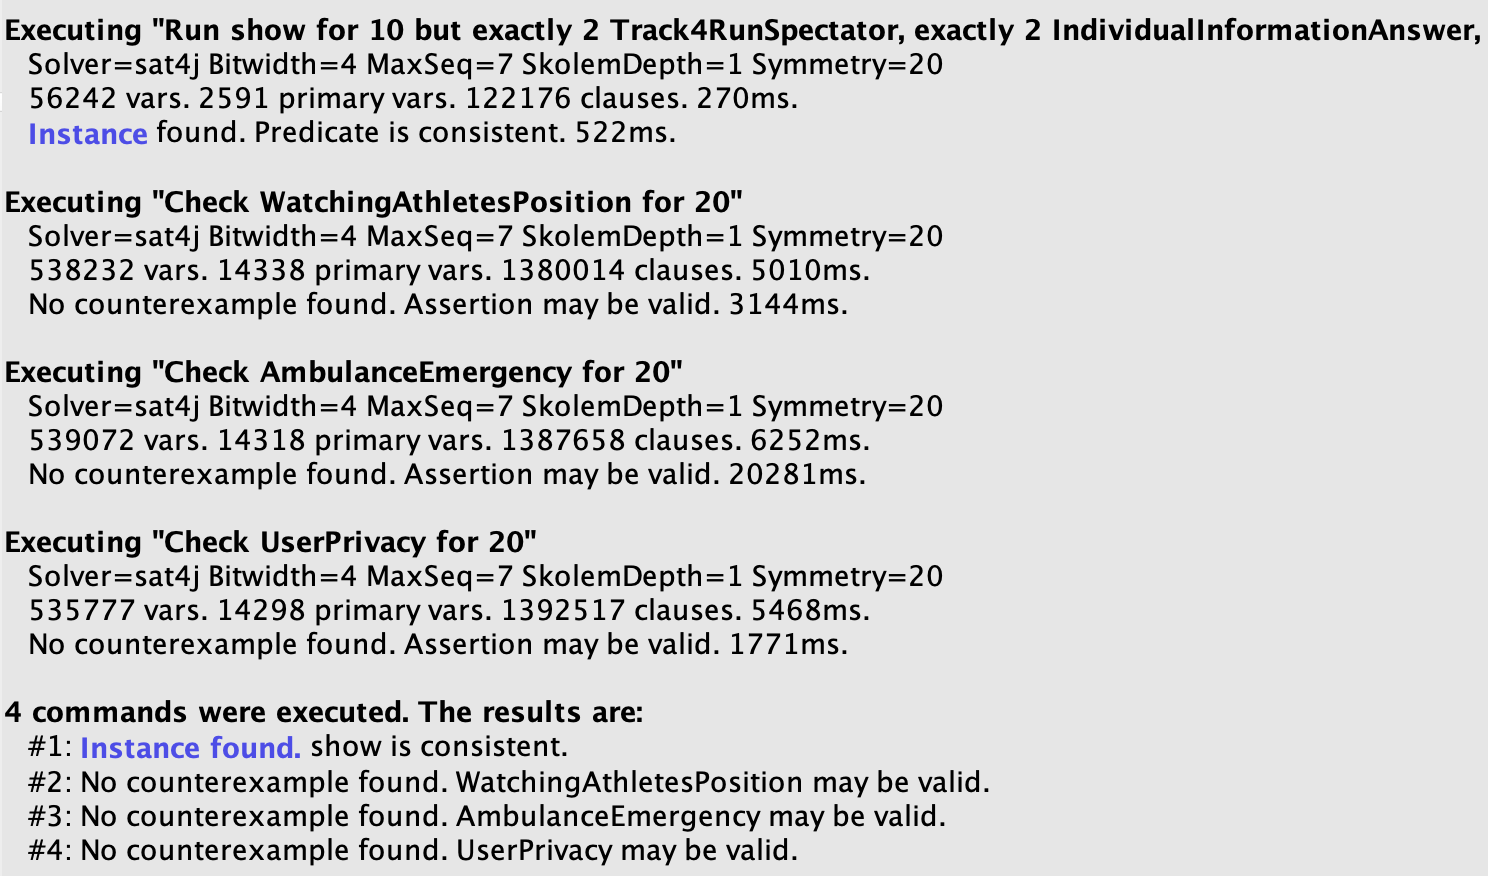
\includegraphics[scale=0.7]{Images/alloyResult.png}
\end{figure}
\subsection{Generated World}
\begin{figure}[H]
\centering
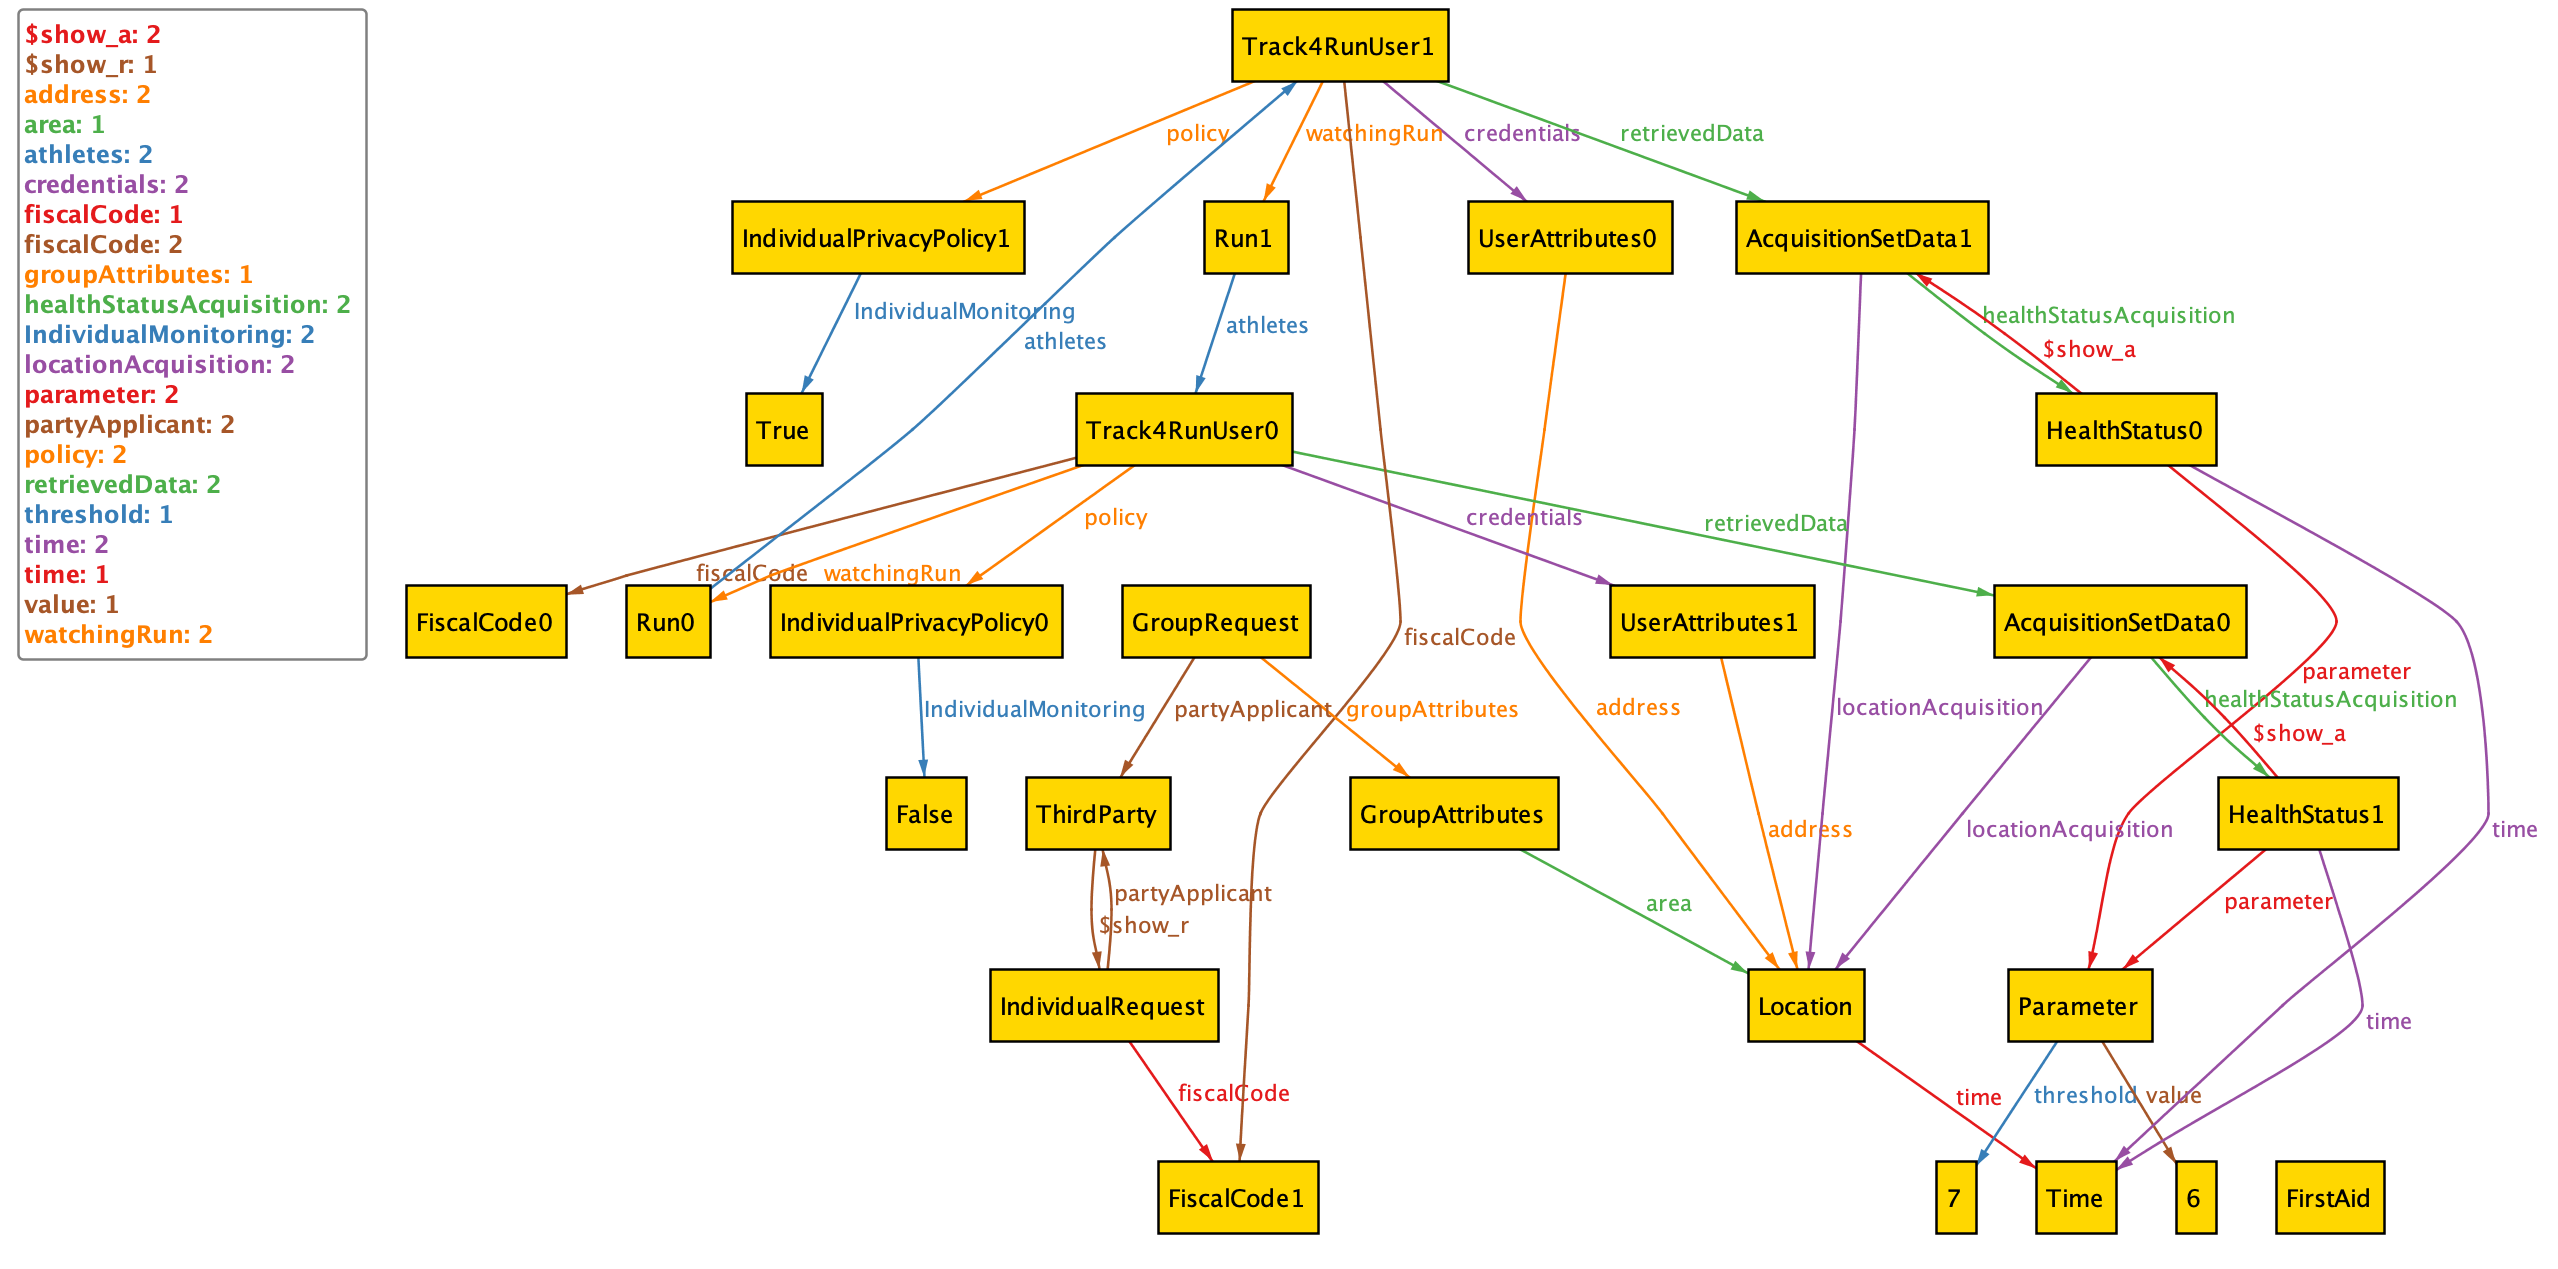
\includegraphics[scale=0.4]{Images/alloyGeneratedWorld.png}
\end{figure}

%------------------------------------------------------------------------------------------------------------------------------------------------
\clearpage
{\color{Blue}{\section{Effort Spent}}}
\label{sect:effort}
This section contains information about how many hours each group member has spent in working at this document.
\bigbreak

\subsubsection{Luca Alessandrelli}
\begin{table}[h]
\centering
\begin{tabular}{|c|c|c|}
\hline
\rowcolor[HTML]{FE996B} 
Date & Task & Hours 
\\ \hline
\rowcolor[HTML]{FFFC9E} 
23/11/18  & Overview & 1  
\\ \hline
\rowcolor[HTML]{FFFC9E} 
24/11/18 & Deployment View & 3  
\\ \hline
\rowcolor[HTML]{FFFC9E}
26/11/18 & Deployment View & 1 
\\ \hline
\rowcolor[HTML]{FFFC9E}
27/11/18 & Runtime View & 6 
\\ \hline
\rowcolor[HTML]{FFFC9E}
29/11/18 & Component Interface & 3
\\ \hline
\rowcolor[HTML]{FFFC9E}
30/11/18 & Runtime View & 2.5
\\ \hline
\rowcolor[HTML]{FFFC9E}
1/12/18 & Component Diagram & 2 
\\ \hline
\rowcolor[HTML]{FFFC9E}
1/12/18 & Runtime View & 1.5
\\ \hline
\rowcolor[HTML]{FFFC9E}
2/12/18 & Deployment View & 0.5
\\ \hline
\rowcolor[HTML]{FFFC9E}
2/12/18 & Component Diagram & 1 
\\ \hline
\rowcolor[HTML]{FFFC9E}
3/12/18 & Implementation,Integration and Test Plan & 5
\\ \hline
\rowcolor[HTML]{FFFC9E}
4/12/18 & Implementation,Integration and Test Plan & 7.5
\\ \hline
\rowcolor[HTML]{FFFC9E}
7/12/18 & Document Revision & 3
\\ \hline

\rowcolor[HTML]{FFCE93} 
\multicolumn{2}{|c|}{Overview} & 1 \\ 
\hline
\rowcolor[HTML]{FFCE93} 
\multicolumn{2}{|c|} {Deployment View} & 4.5 \\
\hline
\rowcolor[HTML]{FFCE93} 
\multicolumn{2}{|c|} {Runtime View} & 10 \\
\hline
\rowcolor[HTML]{FFCE93} 
\multicolumn{2}{|c|} {Component Interface} & 3 \\
\hline
\rowcolor[HTML]{FFCE93} 
\multicolumn{2}{|c|} {Component Diagram} & 3 \\
\hline
\rowcolor[HTML]{FFCE93} 
\multicolumn{2}{|c|} {Implementation,Integration and Test Plan} & 12.5 \\
\hline
\rowcolor[HTML]{FFCE93} 
\multicolumn{2}{|c|} {Document Revision} & 3 \\
\hline



\rowcolor[HTML]{FE996B} 
\multicolumn{2}{|c|}{\cellcolor[HTML]{FE996B}Total} & \cellcolor[HTML]{FFFC9E}37 \\ \hline
\end{tabular}
\caption{Effort Spent Luca Alessandrelli}
\end{table}

\clearpage
\newpage

\subsubsection{Andrea Caraffa}
\begin{table}[h]
\centering
\begin{tabular}{|c|c|c|}
\hline
\rowcolor[HTML]{FE996B} 
Date & Task & Hours 
\\ \hline
\rowcolor[HTML]{FFFC9E} 
26/11/18  & User Interface Design & 4
\\ \hline
\rowcolor[HTML]{FFFC9E} 
27/11/18 & Runtime View & 3 
\\ \hline
\rowcolor[HTML]{FFFC9E}
1/12/18 & Runtime View & 3
\\ \hline
\rowcolor[HTML]{FFFC9E}
1/12/18 & Component Interfaces & 2
\\ \hline
\rowcolor[HTML]{FFFC9E}
2/12/18 & Runtime View & 2
\\ \hline
\rowcolor[HTML]{FFFC9E}
2/12/18 & Component Interfaces & 2
\\ \hline
\rowcolor[HTML]{FFFC9E}
3/12/18 & Runtime View & 1
\\ \hline
\rowcolor[HTML]{FFFC9E}
3/12/18 & Component Interfaces & 1
\\ \hline
\rowcolor[HTML]{FFFC9E}
4/12/18 & User Interface Design & 4
\\ \hline
\rowcolor[HTML]{FFFC9E}
7/12/18 & Implementation Plan & 1
\\ \hline
\rowcolor[HTML]{FFFC9E}
7/12/18 & Integration Plan & 1
\\ \hline
\rowcolor[HTML]{FFFC9E}
7/12/18 & Introduction Section & 3
\\ \hline
\rowcolor[HTML]{FFFC9E}
8/12/18 & User Interface Design & 2
\\ \hline
\rowcolor[HTML]{FFFC9E}
8/12/18 & Document Revision & 6
\\ \hline


\rowcolor[HTML]{FFCE93} 
\multicolumn{2}{|c|}{User Interface Design} & 10 \\ 
\hline
\rowcolor[HTML]{FFCE93} 
\multicolumn{2}{|c|} {Runtime View} & 8 \\
\hline
\rowcolor[HTML]{FFCE93} 
\multicolumn{2}{|c|} {Component Interfaces} & 5 \\
\hline
\rowcolor[HTML]{FFCE93} 
\multicolumn{2}{|c|} {Implementation Plan} & 1 \\
\hline
\rowcolor[HTML]{FFCE93} 
\multicolumn{2}{|c|} {Integration Plan} & 1 \\
\hline
\rowcolor[HTML]{FFCE93} 
\multicolumn{2}{|c|} {Introduction Section} & 3 \\
\hline
\rowcolor[HTML]{FFCE93} 
\multicolumn{2}{|c|} {Document Revision} & 6  \\
\hline


\rowcolor[HTML]{FE996B} 
\multicolumn{2}{|c|}{\cellcolor[HTML]{FE996B}Total} & \cellcolor[HTML]{FFFC9E}34 \\ \hline
\end{tabular}
\caption{Effort Spent Andrea Caraffa}
\end{table}



\FloatBarrier
\clearpage
\newpage
\subsubsection{Andrea Bionda}
\begin{table}[h]
\centering
\begin{tabular}{|c|c|c|}
\hline
\rowcolor[HTML]{FE996B} 
/ & Task & Hours 
\\ \hline
\rowcolor[HTML]{FFCE93} 
\multicolumn{2}{|c|}{Overview} & 3 \\ 
\hline
\rowcolor[HTML]{FFCE93} 
\multicolumn{2}{|c|} {Component Diagram and description} & 15  \\
\hline
\rowcolor[HTML]{FFCE93} 
\multicolumn{2}{|c|} {ER Diagram and description} & 4 \\
\hline
\rowcolor[HTML]{FFCE93} 
\multicolumn{2}{|c|} {Deployment View} & 1 \\
\hline
\rowcolor[HTML]{FFCE93} 
\multicolumn{2}{|c|} {Component interface description} & 1 \\
\hline
\rowcolor[HTML]{FFCE93} 
\multicolumn{2}{|c|} {Architectural styles and patterns} & 5 \\
\hline
\rowcolor[HTML]{FFCE93} 
\multicolumn{2}{|c|} {Requirements traceability} & 10 \\
\hline
%\rowcolor[HTML]{FFCE93} 
%\multicolumn{2}{|c|} {Alloy} & 7 \\
%\hline




\rowcolor[HTML]{FE996B} 
\multicolumn{2}{|c|}{\cellcolor[HTML]{FE996B}Total} & \cellcolor[HTML]{FFFC9E}40 \\ \hline
\end{tabular}
\caption{Effort Spent Andrea Bionda}
\end{table}
\FloatBarrier


%------------------------------------------------------------------------------------------------------------------------------------------------
\clearpage
{\color{Blue}{\section{References}}}
\label{sect:references}
%------------------------------------------------------------------------------------------------------------------------------------------------
\end{document}
